\documentclass{sig-alternate}

\usepackage[utf8]{inputenc}
\usepackage[T1]{fontenc}
\usepackage[T1,T2A]{fontenc}
\usepackage{lmodern}
\usepackage[activate=compatibility]{microtype}

% autoref command
\usepackage[hyphens]{url}
\usepackage[pdftex,urlcolor=black,colorlinks=true,linkcolor=black,citecolor=black]{hyperref}
\def\sectionautorefname{Section}
\def\subsectionautorefname{Subsection}

\usepackage{enumitem}

\usepackage{color}
\definecolor{light-gray}{gray}{0.8}

% todo macro
\usepackage{color}
\newcommand{\todo}[1]{\noindent\textcolor{red}{{\bf \{TODO}: #1{\bf \}}}}

% nicer looking Google+
\usepackage{xspace}
\DeclareRobustCommand{\googleplus}{\mbox{Google\hspace{0em}\raisebox{.28ex}{\tiny\bf +}\kern-0.2ex}\xspace}

% listings and Verbatim environment
\usepackage{fancyvrb}
\usepackage{relsize}
\usepackage{listings}
\usepackage{verbatim}
\newcommand{\defaultlistingsize}{\fontsize{8pt}{9.5pt}}
\newcommand{\inlinelistingsize}{\fontsize{8pt}{11pt}}
\newcommand{\smalllistingsize}{\fontsize{7.5pt}{9.5pt}}
\newcommand{\listingsize}{\defaultlistingsize}
\RecustomVerbatimCommand{\Verb}{Verb}{fontsize=\inlinelistingsize}
\RecustomVerbatimEnvironment{Verbatim}{Verbatim}{fontsize=\defaultlistingsize}
\lstset{frame=lines,captionpos=b,numberbychapter=false,escapechar=§,
        aboveskip=2em,belowskip=1em,abovecaptionskip=0.5em,belowcaptionskip=0.5em,
        framexbottommargin=-1em,basicstyle=\ttfamily\listingsize\selectfont}

% use Courier from this point onward
\let\oldttdefault\ttdefault
\renewcommand{\ttdefault}{pcr}
\let\oldurl\url
\renewcommand{\url}[1]{\inlinelistingsize\oldurl{#1}}

\lstdefinelanguage{JavaScript}{
  keywords={push, typeof, new, true, false, catch, function, return, null, catch, switch, var, if, in, while, do, else, case, break},
  keywordstyle=\bfseries,
  ndkeywords={class, export, boolean, throw, implements, import, this},
  ndkeywordstyle=\color{darkgray}\bfseries,
  identifierstyle=\color{black},
  sensitive=false,
  comment=[l]{//},
  morecomment=[s]{/*}{*/},
  commentstyle=\color{darkgray},
  stringstyle=\color{red},
  morestring=[b]',
  morestring=[b]"
}

% linewrap symbol
\definecolor{grey}{RGB}{130,130,130}
\newcommand{\linewrap}{\raisebox{-.6ex}{\textcolor{grey}{$\hookleftarrow$}}}

\hyphenation{Wikistream Wikipedia Wikipedias}

%\def\baselinestretch{0.99}

\begin{document}

% --- Author Metadata here ---
\conferenceinfo{World Wide Web Conference}{'13 Rio de Janeiro, Brazil}
\CopyrightYear{2013} % Allows default copyright year (20XX) to be over-ridden - IF NEED BE.
%\crdata{0-12345-67-8/90/01}  % Allows default copyright data (0-89791-88-6/97/05) to be over-ridden - IF NEED BE.
% --- End of Author Metadata ---


\title{A Meteoroid on Steroids: Ranking Media Items\\ Stemming from Social Networks}

\numberofauthors{1}\author{
\alignauthor
Thomas Steiner\\
	\affaddr{Google Germany GmbH}\\
	\affaddr{ABC-Str. 19}\\
	\affaddr{20354 Hamburg, Germany}\\
	\email{tomac@google.com} 
}
\maketitle

\begin{abstract}
We have developed an application called Social Media Illustrator
that allows for finding media items on multiple social networks,
clustering them by visual similarity, ranking them by different criteria,
and finally arranging them in aesthetically pleasing media galleries.
In this paper, we focus on the ranking aspect and show how,
for a~given set of media items, the most adequate ranking criterion combination
can be found through interactively applying different criteria
and seeing their effect on-the-fly.
This leads us to an empirically optimized media item ranking formula,
which takes social network interactions into account.
While the ranking formula is not universally applicable,
it can serve as a~good starting point to an individually adapted formula,
all within the context of Social Media Illustrator.
The application is available publicly online at \url{http://social-media-illustrator.herokuapp.com/}.
\end{abstract}

\category{H.3.3}{Information Search and Retrieval}{Clustering}

\terms{Algorithms}

\keywords{}

\section{Introduction}

When people witness events like concerts, sports matches, or meteoroid impacts,
they more and more share media items like photos and videos
that depict these events publicly on social networks.
In the past, we have worked on methods~%
\cite{khrouf2012aggregatingsocialmedia,rizzo2012whatfresh}
for the automatic extraction, deduplication, and clustering of media items
stemming from multiple social networks.
Up to now, we have ordered the retrieved media items chronologically,
by social network, or by cluster size, and thereby completely neglecting
social network interactions as ranking signals.
Though truly added value lies in exploiting these social network interactions
in order to obtain a~more representative ranking of the
potentially many media items retrieved for a~given event.

\section{Related Work}

In~\cite{sanpedro2009ranking}, San Pedro and Siersdorfer propse a~methodology
for automatically ranking and classifying photos from the photo sharing platform Flickr
according to their attractiveness for folksonomy members.
They work with extracted user feedback and annotations available on Flickr
to train machine learning models based on
image features like sharpness and colorfulness.
While their method is tailored to Flickr,
our approach is based on a~social network interaction abstraction layer
on top of the social networks Facebook, Twitter, \googleplus, Instagram,
YouTube, Flickr, MobyPicture, Twitpic, and Lockerz.
Jaffe \emph{et~al.} describe~\cite{jaffe2006generatingsummaries} 
a~ranking and summary algorithm for geo-tagged photo sets based on spatial patterns
as well as textual-topical patterns, and photographer identity cues.
The algorithm can be expanded to support social, temporal, and other factors.
The shown maps-based application necessarily requires geo-tagged media items,
which is rarely the case in media items retrieved from social networks
due to privacy settings and concerns. 
In~\cite{davidson2010youtube}, Davidson \emph{et~al.} describe the different criteria
video quality, user specificity, and diversification
that determine the video ranking in the YouTube recommendation system.
These criteria include view count, the ratings of the video, commenting, favoriting,
and sharing activity around the video.

\begin{figure*}[t!]
  \centering
  \fcolorbox{light-gray}{white}{
  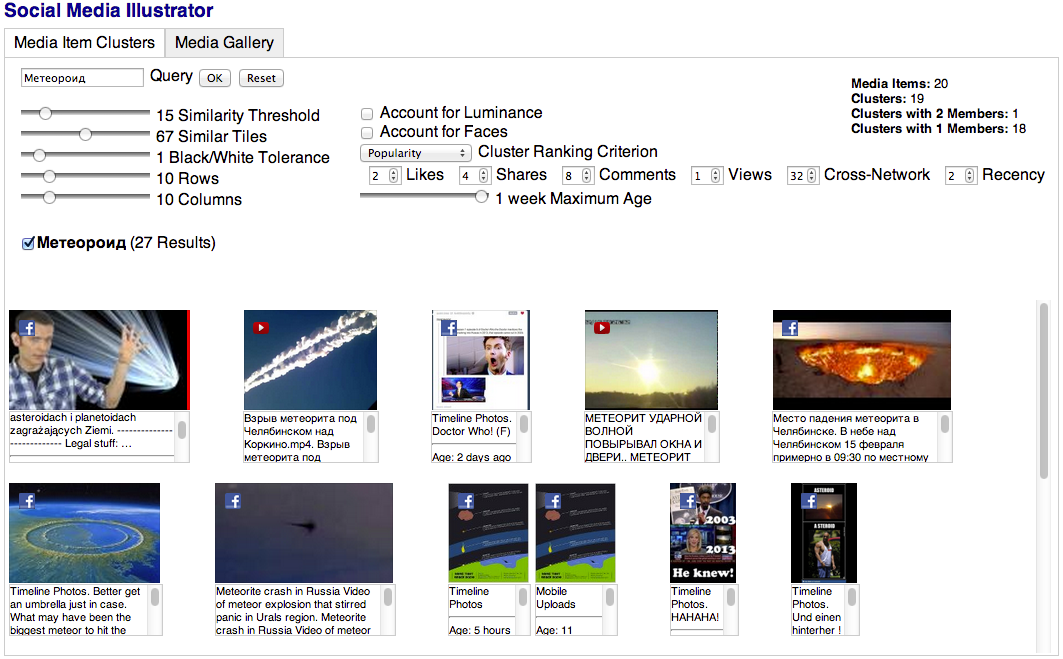
\includegraphics[width=\linewidth]{./application.png}}
  \caption{Media Item Clusters tab of the Social Media Illustrator application
  with individual and clustered (bottom middle) media items from Facebook and YouTube,
  ranked by popularity for the Russian query
    \fontencoding{T2A}\selectfont Метеороид \fontencoding{T1}\selectfont}
  \label{fig:application}
\end{figure*}

\begin{figure*}[t!]
  \centering
  \fcolorbox{light-gray}{white}{
  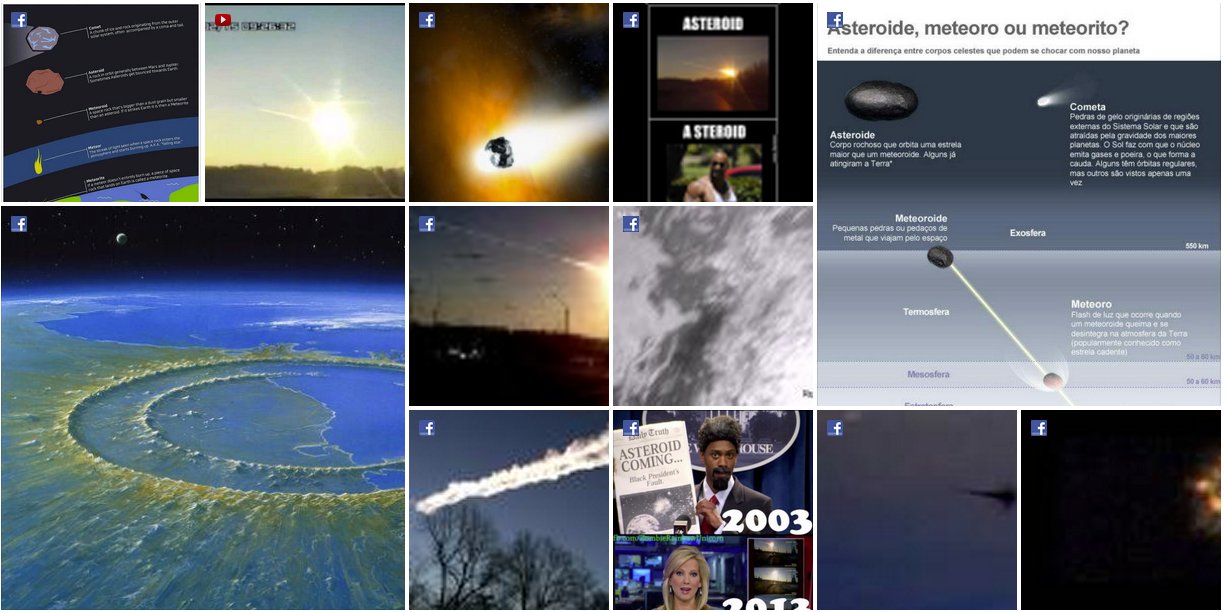
\includegraphics[width=\linewidth]{./media-gallery.png}}
  \caption{Zoomed view of the Media Gallery tab of the application
    showing an automatically generated media gallery in \emph{loose order, varying size} style
    featuring ranked media items stemming from Facebook and YouTube for the query
    \fontencoding{T2A}\selectfont Метеороид \fontencoding{T1}\selectfont}
  \label{fig:media-gallery}
\end{figure*}

\bibliographystyle{abbrv}
\bibliography{www2013devtrack}

\end{document}